\documentclass[11pt,epsf]{article}
\usepackage{graphicx, amssymb, multicol}
\usepackage{fancyhdr, hyperref}


\setlength {\textwidth}{180mm} 
\setlength {\textheight}{232mm}
\topmargin=-6.0mm
\oddsidemargin=-10.0mm
%\pagestyle{empty}
\pagestyle{fancy}
\fancyhf{}
\renewcommand{\headrulewidth}{0pt} % remove lines as well
\lhead{  }
\rhead{  }
%\setcounter{page}{1}
%\cfoot{ }
%\rfoot{ }


\begin{document}

\vspace{-44pt} 
\begin{center}
  {\Large \bf Quasar Science with early {\it James Webb} Observations}
\end{center}

\begin{quotation}
\noindent
{\it  JWST will be cruising to L2 this time in 2018. We better gear up. 
Lorem ipsum dolor sit amet, consectetur adipiscing elit. Aliquam porta
sodales est, vel cursus risus porta non. Vivamus vel pretium
velit. Sed fringilla suscipit felis, nec iaculis lacus convallis
ac. Fusce pellentesque condimentum dolor, quis vehicula tortor
hendrerit sed. Class aptent taciti sociosqu ad litora torquent per
conubia nostra, per inceptos himenaeos. Etiam interdum tristique diam
eu blandit. Donec in lacinia libero.}
\noindent
\end{quotation}

\smallskip
\smallskip
\noindent
{\bf \underline{Introduction.}$\;$}
The link between massive galaxies and the central super-massive black
holes (SMBHs) that seem ubiquitous in them is now thought to be vital
to the understanding of galaxy formation and evolution ([1], [2]).  As
such, huge observational and theoretical effort has been invested in
trying to measure and understand the physics involved in these
enigmatic systems. 

\smallskip
\smallskip
\noindent
Nunc semper quam et leo interdum vulputate eu quis magna. Sed nec arcu
at orci egestas convallis. Aenean quam velit, aliquam vitae viverra
in, elementum vel elit. Nunc suscipit aliquet sapien a suscipit. Cras
nulla ipsum, posuere eu fringilla sit amet, dapibus ultricies
nulla. Nullam eu augue id purus mollis dignissim sed et
libero. Phasellus eget justo sed neque pellentesque egestas nec id
arcu. Donec facilisis pulvinar sapien et fringilla. Suspendisse
vestibulum rhoncus sapien id laoreet. Morbi et orci vitae tortor
imperdiet imperdiet. In hac habitasse platea dictumst. Vivamus vel
neque id mi ultrices tristique. Integer quam libero, ornare vel
gravida in, feugiat a ante. Nam dapibus, tellus vitae pellentesque
cursus, dui nisl egestas augue, non fermentum nisl est nec
nisi. Vestibulum nec mi justo, eget dapibus velit.

\smallskip
\smallskip
\noindent
Cras in laoreet mauris. Vivamus nec nulla a dui commodo
adipiscing. Proin vulputate lectus nec arcu iaculis sit amet auctor
ligula ultricies. Phasellus condimentum gravida tincidunt. Phasellus
et mauris ac nibh vestibulum vehicula. Morbi et augue id purus gravida
sagittis quis in sem. Phasellus quis risus bibendum eros luctus
auctor.

\smallskip
\smallskip
\noindent
Etiam mollis viverra nisi eget aliquet. Aliquam erat volutpat. Vivamus
tristique, nisl eu malesuada semper, libero tortor convallis elit, a
scelerisque orci nisi lacinia turpis. In lacinia ultrices
volutpat. Proin ultrices luctus tellus, in placerat eros tincidunt
id. Ut varius iaculis quam in consequat. Nulla nec orci est, sit amet
pellentesque nisl. Mauris non cursus lectus. Praesent placerat leo vel
erat gravida lacinia. Donec vehicula consectetur lectus vitae
luctus. Praesent nisl justo, laoreet elementum facilisis vel,
tristique ac enim. Etiam vel quam ut quam eleifend
tincidunt. Suspendisse sit amet eros vel elit ullamcorper
laoreet. Etiam venenatis sodales turpis, nec lacinia ligula hendrerit
nec. Nam eu vulputate purus. Quisque facilisis congue metus, sed
imperdiet lorem rhoncus sit amet.

\smallskip
\smallskip
\noindent
Proin non tempus velit. Etiam laoreet, enim nec scelerisque dictum,
tortor massa tempor enim, id pretium justo quam ac lectus. Maecenas
diam nibh, interdum at lobortis sit amet, dignissim et quam. Sed
tincidunt faucibus risus, congue tempus nisl consectetur
eget. Suspendisse venenatis turpis ut risus aliquam interdum. In at
velit sed ligula dictum dignissim ut et dui. Curabitur ac scelerisque
purus.

\smallskip
\smallskip
\noindent
Pellentesque vel elit neque, in interdum lacus. Quisque sodales, nunc
et luctus convallis, nisl dui luctus dui, at congue urna velit a
nisl. Ut sit amet sapien a risus dapibus sagittis. Cras sed ultricies
erat. Donec id metus sed urna lacinia convallis vel sed enim. Proin
nisi libero, ornare vel bibendum eu, sollicitudin sed leo. Cras
tincidunt aliquet ultricies. Cras pretium velit leo, in malesuada
enim. Duis sagittis ultricies interdum. Proin sit amet sem nec metus
feugiat pharetra.

\begin{figure}[h]
  \begin{center}
   \hspace{-0.5cm}
    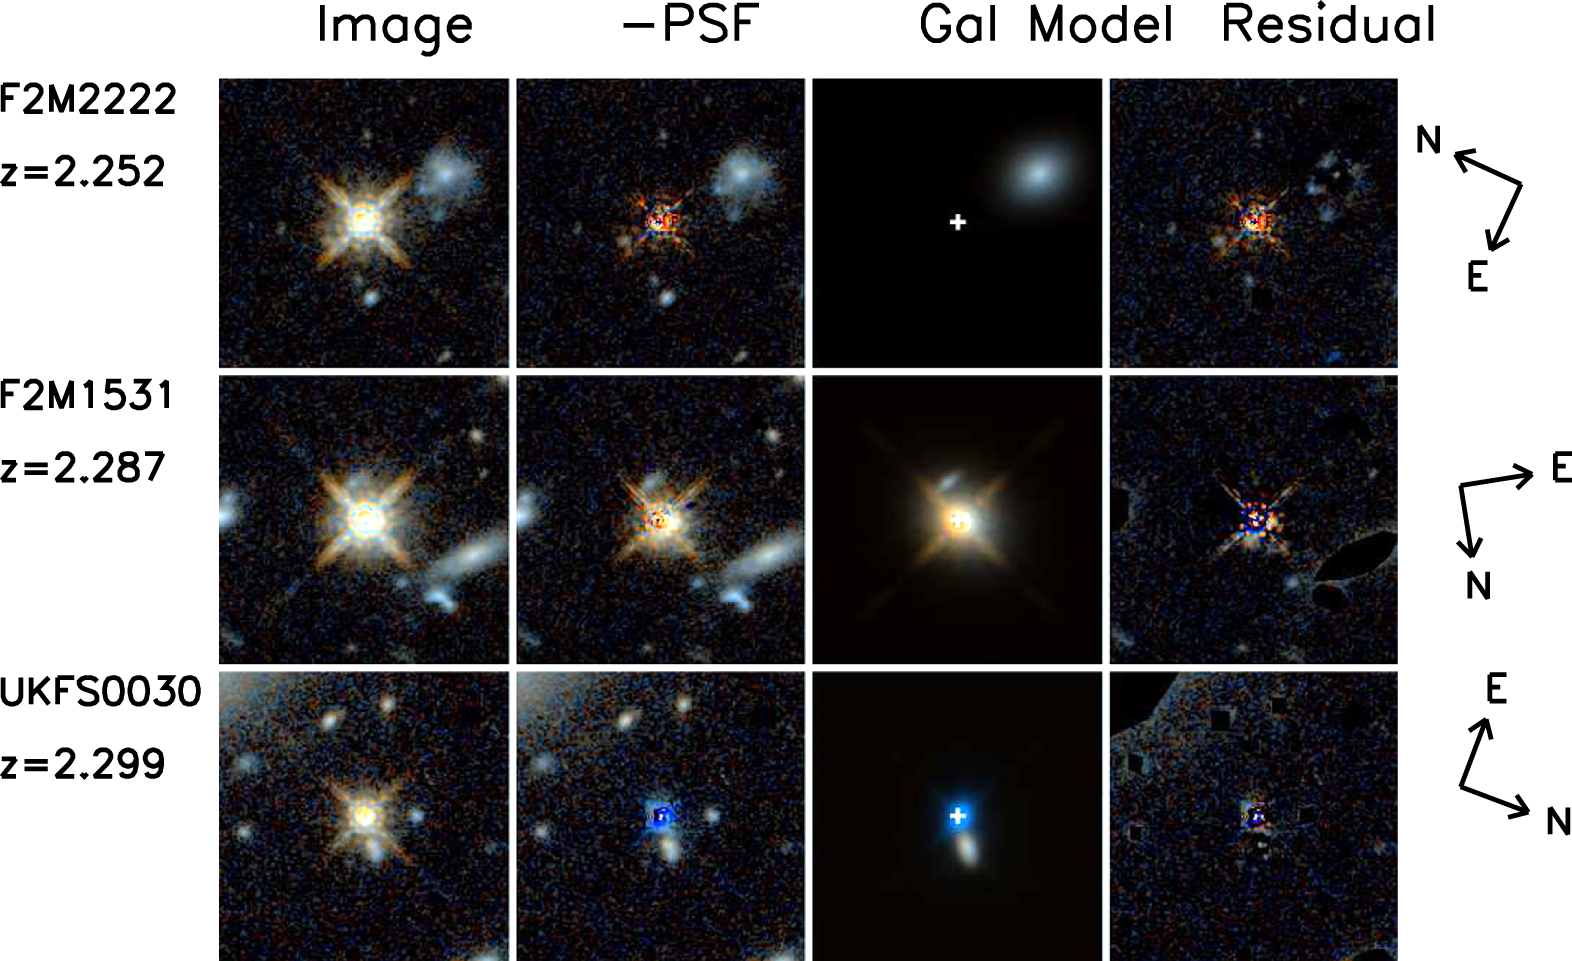
\includegraphics[height=8.5cm,width=16.2cm]
   {figs/Glikman_2015_ApJ_806_218_Fig5_hr.jpg}
%    \vspace{-10pt}
   \caption{     \footnotesize
     {\it From: Glikman et al., 2015, ApJ, 806, 218; their Figure 5.}
     Two color HST images of the eight lower-redshift quasars studied in
     this paper imaged with F105W and F160W. Each row represents a separate
     object. The first column is the original image shown at a scale of 8′′
     × 8′′. The second column shows the residual image after subtracting
     only the point-source component. The third column shows the model for
     all but the point-source component; the blank frame is a source to
     which no host component could be fit. The final panel shows the full
     residual including masked regions and is indicative of the overall
     goodness of fit. Evidence of mergers and disrupted host galaxies is
     seen in most the sources. We apply the red–green–blue color-combining
     algorithm of Lupton et al. (2004) to our images, and we average the
     count rate from the F105W and F160W images to produce the green frame.
}
  \vspace{-14pt}
 \label{figtest-fig}
\end{center}
\end{figure}

\smallskip
\smallskip
\noindent
Aliquam ac metus nec odio tempus pharetra sed nec diam. Sed eget arcu
nulla. Etiam elementum ultrices ligula, at iaculis libero feugiat
bibendum. Suspendisse potenti. Nam pharetra adipiscing
euismod. Quisque imperdiet dignissim odio, sed volutpat justo
tincidunt eu. Nunc vehicula pharetra suscipit. Integer aliquet pretium
ipsum vel ultrices. Nam rutrum nibh ac quam pulvinar molestie.

\smallskip
\smallskip
\noindent
Sed sed ipsum diam. In risus tortor, sagittis eu auctor in, varius in
dui. Mauris a nunc ut ligula ullamcorper tincidunt. Nunc aliquam eros
ac risus pellentesque aliquam. Phasellus augue velit, varius at
porttitor sit amet, pretium eget felis. Ut mollis tellus elementum
magna porttitor rutrum. Etiam blandit leo eget est consectetur
imperdiet. Quisque et diam nec orci vulputate varius vitae id sapien.


\begin{figure}[h]
  \begin{center}
   \hspace{-0.5cm}
    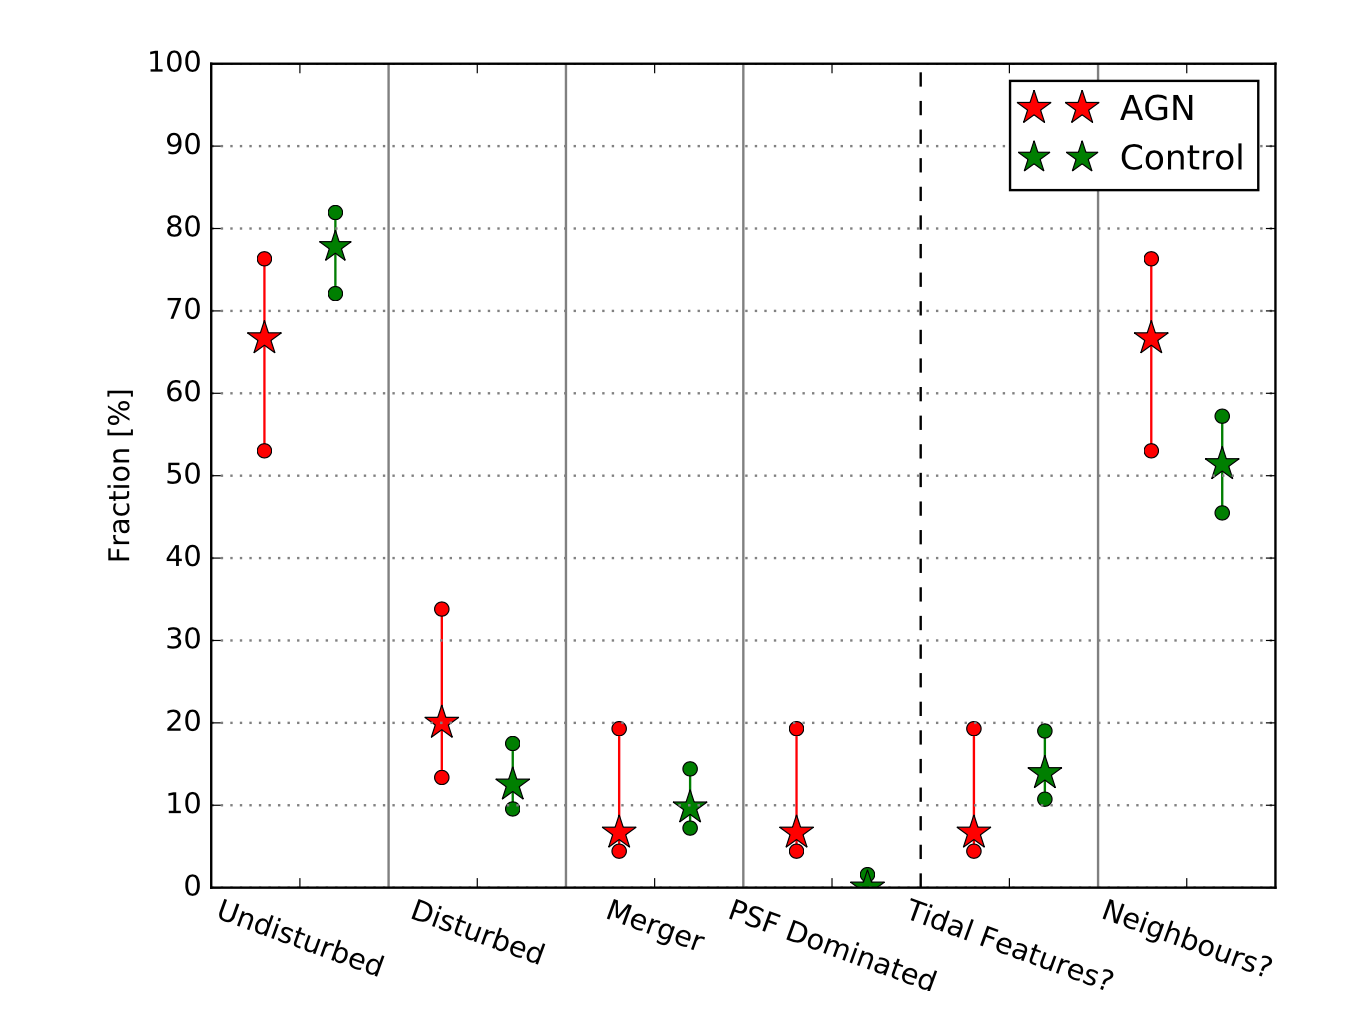
\includegraphics[height=8.5cm,width=12.2cm]
   {figs/Villforth_161106236v2_Fig4_right.png}
    \vspace{-10pt}
   \caption{Villforth et al, arXiv:1611.06236v2; their Figure 4. 
     Visual classification of all resolved AGN host galaxies and
     matched control galaxies. AGN are shown in red, control sample in
     green. The error bars show 1σ confidence intervals calculated
     following Cameron (2011).
}
  \vspace{-14pt}
 \label{figtest-fig}
\end{center}
\end{figure}

%\newpage

%%% 
%%%     \tiny    \scriptsize     \footnotesize     \small     \normalsize     \large    \Large     \LARGE     \huge     \Huge 
%%% 
\smallskip
\smallskip
\noindent
{\bf Mid-IR properties of QSOs and JWST.} 
The discovery of extremely red QSOs (ERQs) with $r~-~[22]~>~14$
colours from the WISE All-Sky Survey and spectroscopy from SDSS and
BOSS, seems to provide a key observational clue to the ``major
merger'' evolutionary theory for QSO activity ([17],[24]).
%% 
However, the large fraction of AGN which remain heavily obscured will
need mid-infrared spectroscopy in order to understand the role this
optically hidden population play in the evolution of galaxies and the
integrated light of the Universe. Given the fellowship timescale, this
makes a natural bridge to the {\it James Webb Space Telescope} and
observations with the Edinburgh-built MIRI spectrograph.

\begin{figure}[h]
  \begin{center}
   \hspace{-0.5cm}
    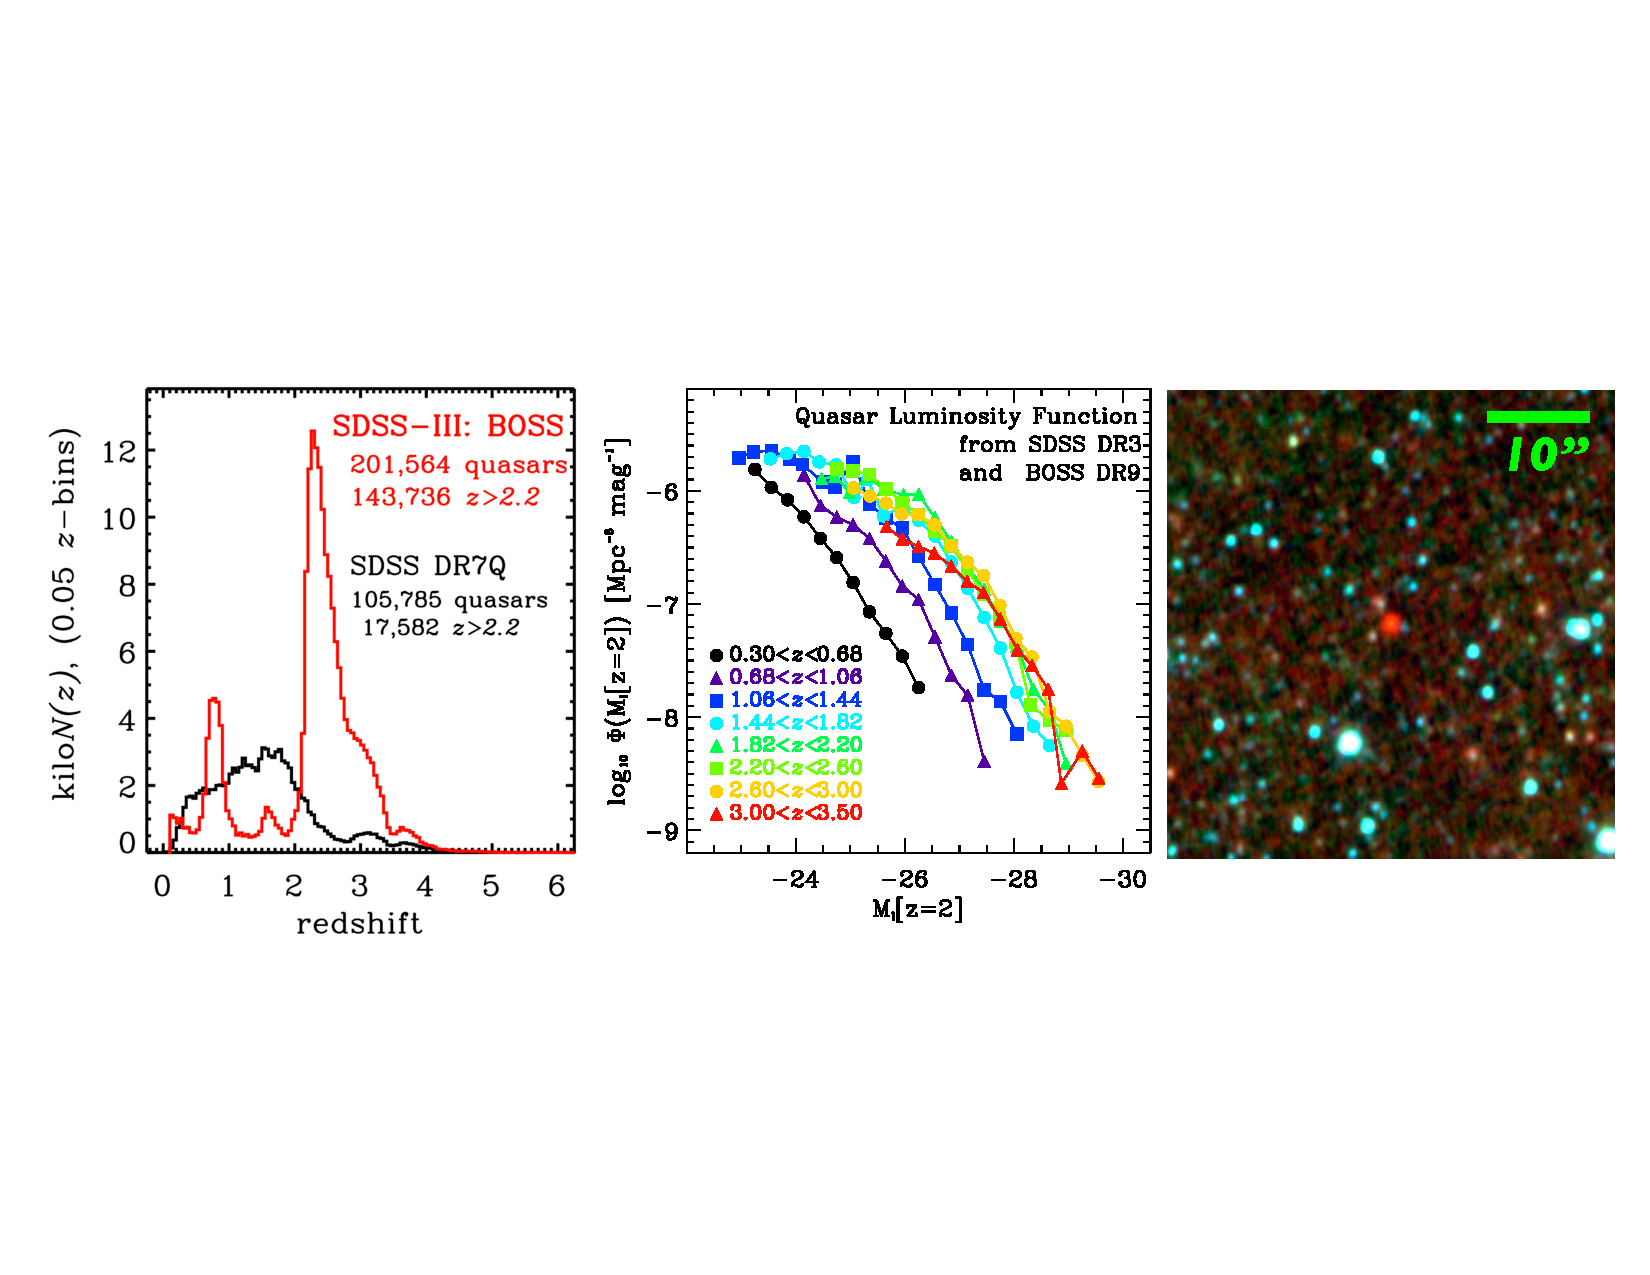
\includegraphics[height=6.5cm,width=18.2cm]
   {figs/3_panels_Nofz_QLF_WISE.pdf}
    \vspace{-10pt}
   \caption{
     \footnotesize
   {\it (Left)} 
   Redshift distributions of QSOs from BOSS (red) and SDSS (black).
    {\it (Centre)}  
    New measurement of the optical QLF from [9] extending the SDSS DR3
    results from [12] and finding a clear break in the QLF at all
    redshifts up to $z=3.5$.
    {\it (Right)} 
    A WISE 3.4, 4.6 and 12$\mu {\rm m}$ image of a $z=2.59$ 
    extremely red QSO, selected on its $r-[22]$ colour. This object
    has a 22$\mu$m flux indicative of $L_{IR} \gtrsim 10^{13.5} L_{\odot}$, 
    and one interpretation could be we are witnessing the
    ``birth'' of an unobscured QSO.  }
  \vspace{-14pt}
 \label{figtest-fig}
\end{center}
\end{figure}


\vspace{-16pt}
\begin{center}
%  {\Large \bf Figures and References \\}
 \medskip
 \medskip
 {\large \bf References}
    \vspace{-10pt}
\end{center}
\begin{multicols}{3}[]
\noindent
%\footnotesize
\scriptsize
%\tiny
\lbrack1\rbrack Fabian, 2012, ARAA, 50, 455 \\
\lbrack2\rbrack Alexander et al., 2012, NewAR, 56, 93\\
\lbrack3\rbrack Schneider et al. 2010, AJ, 139, 2360\\
\lbrack4\rbrack P\^{a}ris et al., 2012, A\&A, 548, A66 \\
\lbrack5\rbrack Dawson et al. 2013, AJ, 145, 10\\
\lbrack6\rbrack Ross et al., 2012, ApJS, 199, 3\\
%\lbrack7\rbrack Busca et al. 2013, A\&A, 522A, 96 \\
%\lbrack8\rbrack Slosar et al., 2013, JCAP, 04, 026 \\
%\lbrack9\rbrack Ross et al., 2013, ApJ, 773, 14, \\
%\lbrack10\rbrack Wright et al., 2010, AJ, 140, 1868\\
%\lbrack11\rbrack P\^{a}ris et al., 2013, A\&A, in prep. \\
%\lbrack12\rbrack Richards et al., 2006, ApJ, 131, 2766\\
%\lbrack13\rbrack Antonucci, 1993, ARA\&A, 31, 473\\
%\lbrack14\rbrack Urry \& Padovani, 1995, PASP, 107, 803\\
%\lbrack15\rbrack Sanders et al.\ 1988, ApJ, 325, 74\\
%\lbrack16\rbrack Canalizo\&Stockton, 2001, ApJ, 555, 719 \\
%\lbrack17\rbrack Hopkins et al., 2006, ApJS, 163, 1\\
%\lbrack18\rbrack White et al., 2012, MNRAS, 424, 933 \\
%\lbrack19\rbrack Geach et al., 2013, arXiv:1307.1706v1\\
%\lbrack20\rbrack Donoso et al., 2013, arXiv:1309.2277v1 \\
%\lbrack21\rbrack Finley et al., 2013, A\&A, accepted\\
%\lbrack22\rbrack Stern et al., 2012, ApJ, 753, 30\\
%\lbrack23\rbrack Assef et al., 2013, ApJ, 772, 26\\
%\lbrack24\rbrack Ross et al. 2013b, MNRAS in advanced prep.
%%Anderson et al. 2012, arXiv:1203.6594v1 \\
%%Banerji et al. 2012, arXiv:1210.6668v1\\
%Busca et al. 2012, arXiv: 1211.2616v1 \\
%Blake et al. 2011, MNRAS, 415, 2892 \\
%Cattaneo et al., 2009, Nature, 460, 213 \\
%Croom et al., 2005, MNRAS, 356, 415 \\
%Coppin et al., 2008, MNRAS, 389, 45 \\
%Croom et al., 2009, MNRAS, 399, 1755 \\
%da \^{A}ngela et al., 2008, MNRAS, 383, 565 \\
%Dawson et al.,  2012, arXiv1208.0022v1 \\ 
%%Dunkley et al., 2011, ApJ, 739, 52 \\
%Eisenstein et al., 2011,  AJ, 142, 72 \\
%Friemann et al. 2008, ARAA, 46, 385 \\
%Fiore et al.,  2011, arXiv1109.2888v1 \\
%Filiz Ak et al. 2012,  ApJ, 757, 114\\
%Haehnelt et al., 1994, MNRAS, 269, 199\\
%Hobbs et al., 2010, CQGra, 27h4013 \\
%Hopkins et al., 2007, ApJ, 654, 731 \\
%Hopkins et al., 2007b, ApJ, 662, 110 \\
%Lang et al., 2009, AJ, 137, 4400 \\
%Li et al, 2011, ApJ, 742, 33 \\
%Lidz et al. 2006, ApJ, 641, 41 \\
%Liu et al., 2011,  ApJ, 737, 101 \\
%Lonsdale et al., 2003, PASP, 115, 897\\
%Mauduit et al., 2012, PASP, 124. 714\\
%Palanque-Delabrouille~et~al., 2012, arXiv1209.3968v1 \\
%Palanque-Delabrouille~2012, arXiv1209.3968v1 \\
%P\^{a}ris, et al. 2012,  arXiv1210.5166v1\\
%Peth et al. 2011, AJ, 141, 105 \\
%Richards et al, 2006, AJ, 131, 2766 \\
%Ross et al., 2007, MNRAS, 381, 573  \\
%Ross et al., 2008, MNRAS, 387, 1323 \\
%Ross et al., 2009, ApJ, 697, 1634 \\
%Ross et al., 2012b, arXiv:1210.6389v1 \\
%Ross et al., 2012c, ApJL, in prep.\\
%Sanders et al. 2007, ApJS, 172, 86 \\ 
%Sawangwit~et~al.~2011,~arXiv:1108.1198v2 \\
%Schlegel et al., 2009, arXiv:0902.4680v1 \\
%Schneider et al., 2007,  AJ, 134, 102 \\
%Schneider et al., 2010,  AJ, 139, 2360 \\
%Seljak et al. 2009,  PhRvL, 091303\\
%Sesana et al., 2008, MNRAS, 390, 192 \\
%Simmons et al., 2011, ApJ, 734, 121 \\
%Shen et al. 2007, AJ, 133, 2222  \\
%Shen et al. 2009, ApJ, 697, 1656 \\
%Slosar et al, 2011, JCAP, 09, 1 \\
%Thorne, {\it Gravitational Radiation} 1987 \\
%White, astro-ph/0305474v1 \\

%Wang et al., 2009, ApJ, 697, L141 \\
%Wardlow et al., 2011, MNRAS, 415, 1479 \\
\end{multicols}


\end{document}
